\documentclass[11pt,letterpaper]{article}
\usepackage{geometry}
\geometry{margin=1in}

\usepackage{graphicx}
\usepackage{caption}   % for better caption control
\usepackage{float}     % to control image placement
\usepackage{parskip}   % to add spacing between paragraphs
\usepackage[hidelinks]{hyperref}
\usepackage{amsmath}
\usepackage{amsmath}
\usepackage{amsfonts} 
\usepackage{minted}
\usepackage{mathtools}
\usepackage{cancel}
\usepackage{subcaption}
\usepackage[thinc]{esdiff}
\usepackage{listings}
\usepackage[framed , numbered]{matlab-prettifier}
\usepackage{bm}
\usepackage{graphicx}
\usepackage{siunitx}
\usepackage{tikz}
\usepackage{booktabs}
\usepackage{hyperref}
\usepackage{tabularx}
\usepackage{url}

\setlength{\parindent}{0pt}
\setlength{\parskip}{0.5em}

% Lists and spacing
\usepackage{enumitem}
\setlist{nosep}

% Reduce section spacing
\usepackage{titlesec}
\titlespacing*{\section}{0pt}{0\baselineskip}{0.5\baselineskip}
\titlespacing*{\subsection}{0pt}{0\baselineskip}{0.3\baselineskip}
\titlespacing*{\subsubsection}{0pt}{0\baselineskip}{0.3\baselineskip}

\title{Lab 3.2 - FMRI, Stat 214, Spring 2025\vspace{-1em}}
\author{Anonymous}

% submission must not contain any of your names
% but feel free to make a version for yourself with your names on it
% \author{Your names}

\begin{document}
\maketitle

\vspace{1em} % space before
\section{Introduction}
\vspace{0.5em} % space after

The ability to model and predict brain activity in response to language is a central challenge in both cognitive neuroscience and machine learning. Human language processing is inherently complex, involving dynamic, context-dependent representations that evolve across time and semantic structures. Traditional approaches to bridging language and brain signals have relied on static word embeddings, such as Bag-of-Words (BoW), Word2Vec, or GloVe, which offer limited capacity to capture contextual nuances or adapt to specific linguistic environments. In Lab 3.2, we address these limitations by developing a custom-trained transformer-based encoder, designed to generate language embeddings that are specifically tailored to the stimuli used in an fMRI study.

This lab builds on the foundation established in Lab 3.1, where pre-trained embeddings were used to predict voxel-wise BOLD (Blood Oxygen Level Dependent) responses. While useful, those embeddings were trained on general corpora unrelated to the spoken podcast narratives presented during the fMRI recordings. As a result, they may fail to capture task-specific linguistic patterns relevant to neural responses. To overcome this, Lab 3.2 leverages advances in self-supervised learning, particularly Masked Language Modeling (MLM), to pre-train an encoder directly on the same podcast transcripts heard by participants. MLM enables the model to learn rich, contextualized representations without requiring labeled data, making it an ideal strategy for domains where supervised labels—like brain responses—are expensive or sparse.

The importance of this work extends beyond technical implementation. By aligning language representations more closely with the actual stimuli that elicited neural activity, we aim to improve both predictive accuracy and scientific interpretability. Custom embeddings trained on task-relevant data have the potential to reveal deeper insights into how the brain encodes semantic and syntactic information. Furthermore, this lab highlights the practical value of domain adaptation in machine learning—showing that models fine-tuned on context-specific data often outperform generic solutions.

Lab 3.2 is structured in two key phases. First, we implement the encoder architecture and conduct pre-training using MLM, experimenting with various hyperparameters such as learning rate, batch size, and sequence length. We carefully monitor training and validation loss curves to evaluate convergence and prevent overfitting. Second, we apply the embeddings generated by our pre-trained encoder to predict voxel-level fMRI responses using ridge regression, replicating the modeling pipeline from Lab 3.1. A detailed comparative analysis is conducted to assess how our task-specific embeddings perform relative to standard pre-trained methods.

\vspace{1em} % space before
\section{Pre-Training}
\vspace{0.5em} % space after

To generate task-specific language embeddings for neural response prediction, we pre-trained a custom transformer-based encoder using a MLM objective. MLM enables the model to learn contextualized representations by randomly masking a portion of input tokens and training the encoder to predict them based on surrounding context. This self-supervised approach allowed the encoder to capture semantic and syntactic patterns directly from the podcast transcripts that were used as stimuli during the fMRI recordings. By training on the same linguistic data heard by participants, the encoder was better positioned to produce embeddings aligned with the neural processes involved in language comprehension.

The pre-training process was implemented using the provided train\_encoder.py framework, which handled token masking and optimization using cross-entropy loss. The dataset was tokenized using a BERT tokenizer, and various hyperparameters—such as learning rate, batch size, and number of epochs—were explored to ensure effective learning. Training and validation losses were tracked across epochs to evaluate model performance and prevent overfitting. The resulting encoder produced contextual embeddings tailored to the task, which were later applied in downstream modeling to predict voxel-wise brain activity. This pre-training phase was essential for adapting the encoder to the specific linguistic environment, aiming to improve predictive performance over generic, pre-trained embeddings.

\vspace{1em} % space before
\subsection{Implement encoder model}
\vspace{0.5em} % space after

To generate task-specific contextual embeddings for fMRI prediction, we implemented a custom Transformer-based encoder architecture. The encoder was designed to follow the general structure of BERT encoders while adapting to the scale and needs of the current dataset.

The encoder consists of three primary embedding layers: token embeddings, position embeddings, and segment type embeddings. Each input token is mapped into a dense vector via the token embedding layer, with additional positional information added through a learned position embedding. Type embeddings are incorporated to differentiate between different segments, though in our case most inputs were single sequences.

The embedded input is passed through a stack of Transformer blocks. Each Transformer block contains two key submodules:

\begin{itemize}
    \item A \textbf{Multi-Head Self-Attention} layer, implemented using PyTorch’s \verb|MultiheadAttention| module with batch-first inputs, which allows the model to jointly attend to information from different subspaces of representation.
    \item A \textbf{Feed-Forward Neural Network} with an intermediate hidden layer and ReLU activation, applied independently to each position.
\end{itemize}
Each submodule is wrapped with a residual connection and layer normalization to promote stable and efficient training. A final layer normalization is applied after the entire stack of Transformer blocks to normalize the output hidden states.

For the pre-training objective, a Masked Language Modeling head was added on top of the encoder. This head projects the final hidden states back into the vocabulary space, allowing the encoder to predict masked tokens during training. After pretraining, only the hidden states, not the MLM predictions, were used as contextual embeddings for downstream fMRI modeling.

The encoder was designed with flexibility to experiment with different hyperparameters, including hidden size, number of attention heads, number of layers, and feed-forward intermediate size. Following a detailed hyperparameter tuning process (Section 2.3), we selected a lightweight configuration with 128 hidden dimensions, 2 Transformer layers, and 4 attention heads, which achieved optimal trade-off between learning capacity and overfitting risk on the available podcast transcript data.

\vspace{1em} % space before
\subsection{Implement masked-language model training}
\vspace{0.5em} % space after

To enable the encoder to learn meaningful, contextualized language representations, we implemented a MLM training procedure within train\_encoder.py. MLM is a self-supervised learning technique where a portion of input tokens is randomly masked, and the model is trained to predict these masked tokens using contextual cues from surrounding words. This approach forces the encoder to develop a deep understanding of language structure and semantics without requiring labeled data, making it ideal for pre-training on the podcast transcripts used in this study.

The core of this implementation involved two key components: the mask\_tokens function and the train\_bert training loop. The mask\_tokens function was designed to follow standard MLM practices—randomly selecting 15\% of tokens for prediction, replacing 80\% of them with a MASK token, 10\% with random tokens, and leaving the remaining 10\% unchanged. Special care was taken to ensure that padding tokens were excluded from masking, and all operations were optimized for GPU computation by explicitly handling device placements.

The train\_bert function handled the full training pipeline, including dataset management, optimization, and loss computation. To ensure robust evaluation, we incorporated an automatic train-validation split within the function, allocating 10\% of the data for validation. This allowed us to monitor both training and validation losses across epochs, providing insight into model convergence and generalization. The model was trained using the Adam optimizer with a cross-entropy loss function applied to the masked token predictions. Attention was given to handling tensor dimensions appropriately, especially when reshaping logits and labels for loss calculation in a multi-class setting over the vocabulary space.

By integrating validation tracking and automating the masking process within each batch, this implementation provided a flexible framework for efficient MLM pre-training. The resulting setup allowed us to experiment with different encoder architectures and hyperparameters while ensuring consistent training dynamics. This foundational work was critical in preparing the encoder to generate high-quality, task-specific embeddings for downstream fMRI prediction tasks in the subsequent phases of the lab.

\vspace{1em} % space before
\subsection{Result of pre-training}
\vspace{0.5em} % space after

\begin{figure}[H]
    \centering
    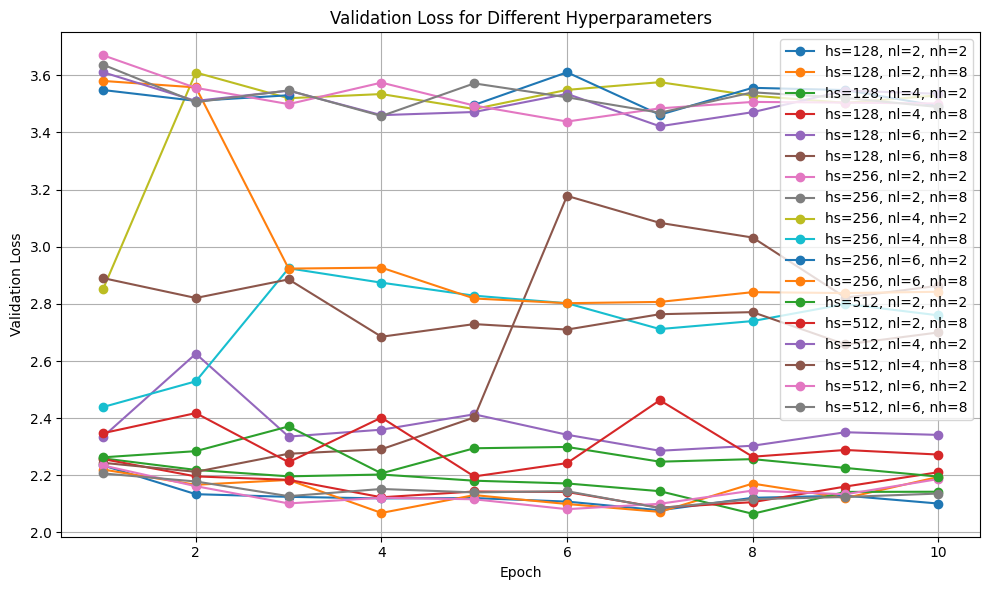
\includegraphics[width=0.9\textwidth]{figs/val_loss_graph.png}
    \caption{Validation Loss for Different Hyperparameters}
    \label{fig:prob_hist_glove}
\end{figure}

\begin{table}[h!]
\centering
\begin{tabular}{|c|c|c|}
\hline
\textbf{Epoch} & \textbf{Train Loss} & \textbf{Val Loss} \\
\hline
1  & 2.3682 & 2.1924 \\
2  & 2.1804 & 2.1886 \\
3  & 2.1357 & 2.1551 \\
4  & 2.1330 & 2.1248 \\
5  & 2.1025 & 2.0828 \\
6  & 2.0981 & 2.1316 \\
7  & 2.0793 & 2.0886 \\
8  & 2.0592 & 2.1247 \\
9  & 2.0850 & 2.0973 \\
10 & 2.0698 & 2.0944 \\
\hline
\end{tabular}
\caption{Training and Validation Loss per Epoch for BEST Encoder (hs=128, nl=2, nh=2)}
\label{tab:best_encoder_loss}
\end{table}

To pre-train the custom transformer-based encoder using Masked Language Modeling (MLM), we conducted an extensive hyperparameter search aimed at identifying the best architecture for modeling the podcast dataset. In this tuning phase, we varied three key parameters: the hidden size (128, 256, 512), the number of layers (2, 4, 6), and the number of attention heads (2, 8). Other settings were held constant: the learning rate was fixed at 3e-4, batch size was 32, and intermediate feedforward size was set to 512. Each configuration was trained for 10 epochs, and both training and validation losses were monitored to assess model performance.

The validation loss curves across different hyperparameter combinations are shown in Figure 1. The results demonstrate that models with larger hidden sizes and deeper architectures tended to exhibit higher validation losses, suggesting overfitting or excessive model capacity relative to the training data size. For instance, architectures with hidden size 512 consistently showed validation losses above 3.0 throughout training. On the other hand, smaller models with hidden size 128 and fewer layers (e.g., 2 or 4) achieved significantly lower validation losses, indicating better generalization. The number of attention heads also influenced results; increasing attention heads to 8 sometimes degraded performance, particularly in larger models, likely due to over-parameterization.

After evaluating all configurations, the best-performing model was found to have a hidden size of 128, 2 transformer layers, and 2 attention heads. This model achieved the lowest validation loss (~ 2.09) after 10 epochs of training, as shown in Table 1. Additionally, the training and validation losses remained relatively close throughout training, suggesting that the model generalized well without significant overfitting. The selected encoder was subsequently retrained on the full training dataset using these best hyperparameters and saved for use in downstream modeling.

The hyperparameter tuning process confirmed that simpler architectures were better suited for this domain-specific corpus. Models with fewer layers, smaller hidden sizes, and fewer attention heads consistently outperformed their larger counterparts, particularly in terms of validation loss and training stability. This outcome aligns with theoretical expectations: the podcast transcript dataset, while linguistically meaningful, is relatively limited in size and diversity compared to large-scale datasets typically used in pretraining models like BERT or GPT. In such cases, larger models tend to overfit or underutilize their capacity, leading to suboptimal generalization.

Additionally, smaller architectures have the advantage of faster training, reduced memory requirements, and more interpretable behavior—all of which are desirable in a neuroscience-focused pipeline where efficiency and model transparency are often critical. The chosen best encoder (with hidden size 128, 2 layers, and 2 attention heads) demonstrated that a lightweight model was sufficient to learn high-quality contextual representations, effectively capturing local and global linguistic patterns in the stimulus without introducing instability or unnecessary complexity. These findings reinforce the importance of tailoring model capacity to the specific scale and nature of the available data, especially when the goal is to extract interpretable features for downstream cognitive modeling tasks.

\newpage
\vspace{1em} % space before
\section{Modeling \& Evaluation}
\vspace{0.5em} % space after
After pre-training the transformer-based encoder, the next phase involved applying the encoder to generate embeddings and predict brain activity responses using ridge regression.

\vspace{1em} % space before
\subsection{Modeling}
\vspace{0.5em} % space after
% Connor
Using the best pretrained encoder, we first generated sentence-level embeddings for all podcast stories in the dataset. Each story was tokenized using a BERT tokenizer, and the input sequences were fed through the encoder to obtain hidden states for each token. To produce a single embedding per text chunk, we computed the mean of the hidden states across the sequence length.

As with previous experiments in Lab 3.1, it was necessary to align the temporal resolution of the embeddings with the fMRI data. Thus, the embeddings were downsampled to match the sampling rate of the BOLD signal. To minimize boundary artifacts, we trimmed the first 5 seconds and last 10 seconds of each story. Finally, we generated lagged features by applying delays of 1 to 4 seconds to the downsampled embeddings. This ensured that the model had access to information from previous timepoints, accounting for the hemodynamic delay inherent in fMRI signals. These final processed embeddings then serves as the final input features for the modeling stage, identical to Lab 3.1. With the encoder-derived embeddings prepared, we trained a ridge regression model to predict voxel-wise fMRI responses.

The data was split into a training set and a held-out test set at the story level. Only training stories were used to fit the model, and performance was evaluated exclusively on unseen test stories to ensure a proper assessment of generalization.

To select the optimal regularization strength for the ridge model, we conducted a 5-fold cross-validation procedure on a random 10\% subsample of the training data. Rather than searching over a broad range of values, we restricted the candidate set to 
$\alpha \in (1, 10, 100, 1000, 10000)$
to focus on reasonable levels of regularization. Cross-validation was performed using negative mean squared error as the scoring metric. The value of $\alpha$ that minimized the validation error was 10000 and the model was then retrained on the full cleaned training set using the best $\alpha$

\vspace{1em} % space before
\subsection{Evaluation}
\vspace{0.5em} % space after
% Connor
The ridge regression model was trained using the aforementioned embeddings derived from the raw podcast transcripts.  The final training data consisted of 28,644 timepoints and 512 features across all usable stories.

The model's performance was evaluated on held-out test stories using voxel-wise Pearson correlation coefficients (CC) between predicted and actual BOLD signals. As shown in Figure \ref{fig:prob_hist_custom}, the resulting CC distribution was centered near zero, with a mean CC of 0.0060 and a median of 0.0054. Only a small subset of voxels showed modest predictive performance, with the top 1\% and top 5\% reaching 0.0466 and 0.0318, respectively. These results suggest that while our custom trained embeddings captures some minimal information about brain responses to language, its representation may lack the semantic richness required for accurate neural encoding.

\begin{table}[H]
\centering
\begin{tabular}{lcccc}
\toprule
\textbf{} & \textbf{Value} \\
\midrule
Mean CC    & 0.0060 \\
Median CC  & 0.0054 \\
Top 1\% CC & 0.0466 \\
Top 5\% CC & 0.0318 \\
\bottomrule
\end{tabular}
\caption{Ridge Regression Model Performance (Subject 2)}
\label{tab:custom_cc_results}
\end{table}

\begin{figure}[ht]
    \centering
    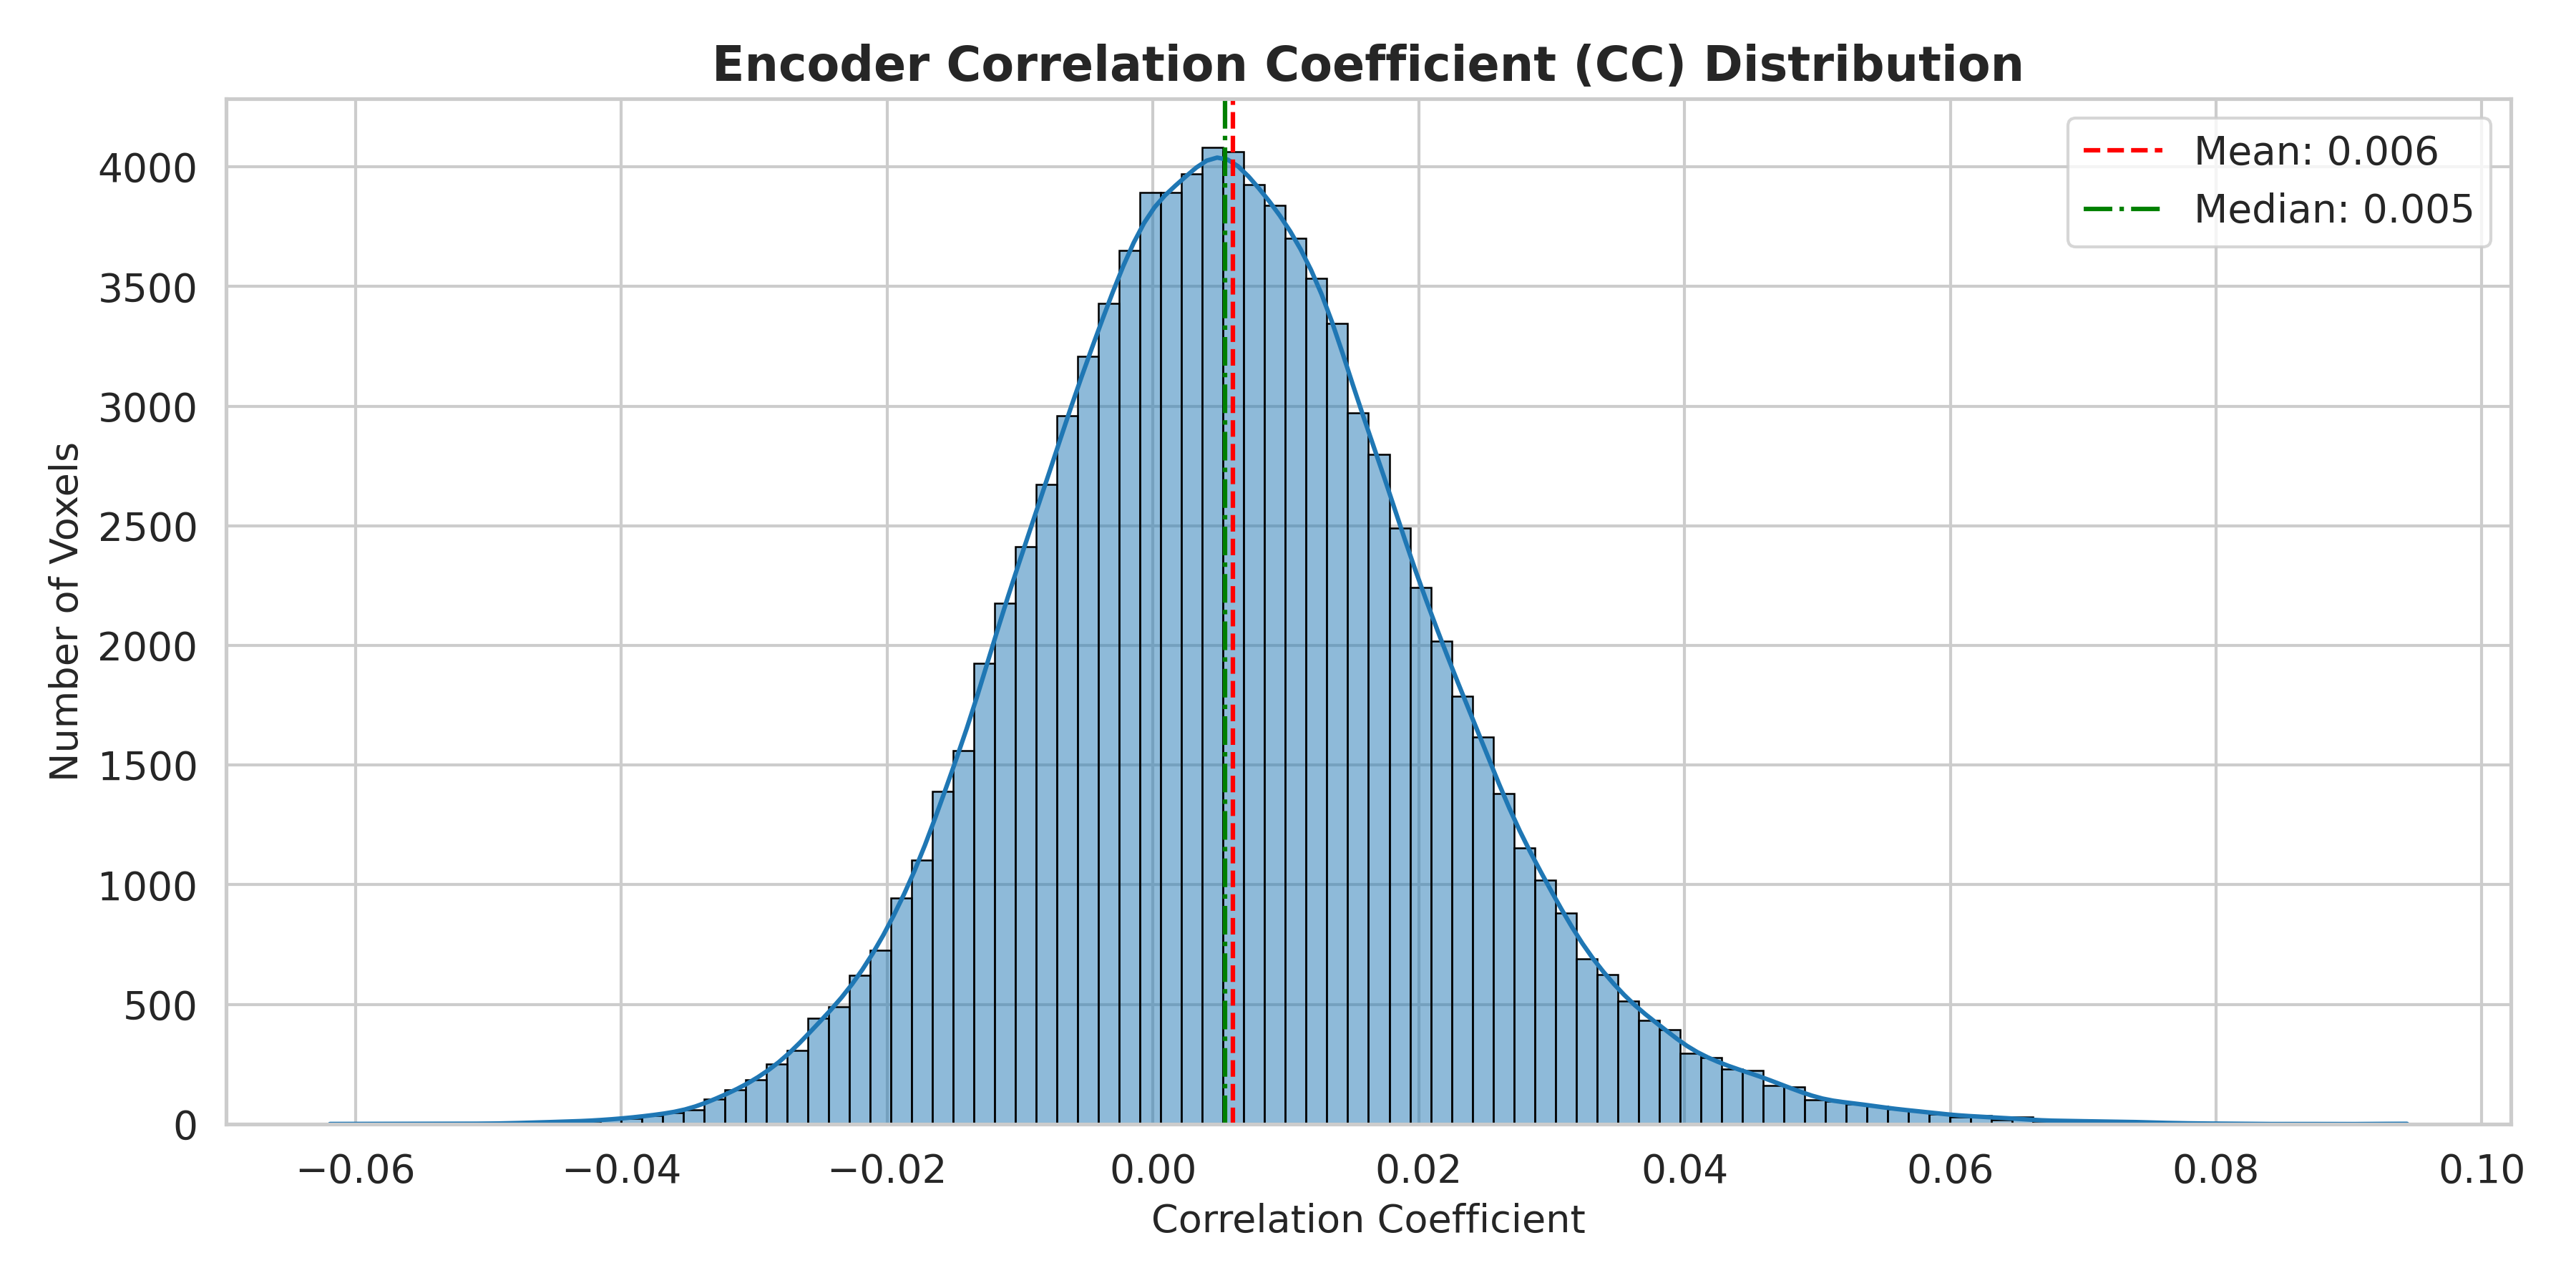
\includegraphics[width=0.9\textwidth]{figs/cc_distribution__trained_encoder_subject2.png}
    \caption{Correlation Coefficient Distribution}
    \label{fig:prob_hist_custom}
\end{figure}


\vspace{1em} % space before
\subsection{Comparison with Lab 3.1}
\vspace{0.5em} % space after
In Lab 3.1, we employed pre-trained embeddings such as Bag-of-Words (BoW), Word2Vec, and GloVe to predict voxel-wise fMRI responses, while in Lab 3.2, we trained a custom encoder to generate our own embeddings. Comparing the performance between the two labs, we observe that the correlation coefficients (CCs) achieved by the self-trained encoder are slightly lower than those achieved by GloVe in Lab 3.1. Specifically, from the distribution plots, the mean CC for the encoder model is around 0.006, while GloVe embeddings reached a mean CC of approximately 0.008. Similarly, the median CC dropped from about 0.007 (GloVe) to 0.005 (encoder). These results suggest that while our self-trained encoder captures some meaningful information from the text, it has not yet surpassed the performance of large-scale pre-trained models such as GloVe.

\begin{table}[H]
\centering
\begin{tabular}{lcc}
\hline
\textbf{Experiment} & \textbf{Mean CC} & \textbf{Median CC} \\
\hline
Lab 3.1 (The best embeddings) & 0.008 & 0.007 \\
Lab 3.2 (Customized embeddings) & 0.006 & 0.005 \\
\hline
\end{tabular}
\caption{Comparison of Mean and Median Correlation Coefficients between Lab 3.1 and Lab 3.2 }
\label{tab:cc_comparison}
\end{table}

In terms of stability, both labs conducted per-story evaluations. The violin plots reveal that the distributions of voxel-wise CCs across different test stories are similarly centered around zero, with a small positive skew in both cases. However, the spread for the encoder-trained features is slightly tighter than that observed for BoW and GloVe, indicating better consistency across different stories, even though the overall CC level is lower. This suggests that the encoder produces embeddings that are more uniformly stable across different narratives but are slightly weaker in absolute predictive power compared to heavily pre-trained embeddings.

\begin{figure}[H]
\centering
\begin{minipage}{0.48\textwidth}
    \centering
    \includegraphics[width=\linewidth]{figs/Stability Check(lab3.1).png}
    \caption*{(a) Lab 3.1 (GloVe Stability Check)}
\end{minipage}
\hfill
\begin{minipage}{0.48\textwidth}
    \centering
    \includegraphics[width=\linewidth]{figs/Stability Check(lab3.2).png}
    \caption*{(b) Lab 3.2 (Own Encoder Stability Check)}
\end{minipage}
\caption{Comparison of Stability Check Results between Lab 3.1 (GloVe) and Lab 3.2 (Own Encoder)}
\label{fig:stability_comparison}
\end{figure}

In conclusion, while the custom encoder offers encouraging stability across stories, it currently underperforms compared to established embeddings in terms of raw voxel prediction accuracy. Future improvements could involve scaling up the training corpus or optimizing model capacity to better match the pre-trained embeddings' effectiveness.

\newpage
\sloppy
\section{Bibliography}

[1] Jain, Shain, and Alexander G. Huth. “Incorporating Context into Language Encoding Models for fMRI.” Proceedings of the 32nd International Conference on Neural Information Processing Systems (NeurIPS), 2018, pp. 6628–6637. \url{https://proceedings.neurips.cc/paper_files/paper/2018/file/5cfb4e6e63a23722cc1a26e3027b8de2-Paper.pdf}.

[2] Li, Xiu, et al. “Evaluating Embeddings from Pre-Trained Language Models and Knowledge Graphs for Educational Content Recommendation.” Future Internet, vol. 16, no. 1, 29 Dec. 2023, pp. 12–12, \url{www.mdpi.com/1999-5903/16/1/12, https://doi.org/10.3390/fi16010012.}

\appendix

\vspace{1em} % space before
\section{Academic honesty}

\vspace{1em} % space before
\subsection{Statement}
\vspace{0.5em} % space after

We are committed to upholding the highest standards of academic integrity in every aspect of our work. We pledge to properly acknowledge all sources, avoid plagiarism, and ensure that our contributions—whether individual or collaborative—are original, transparent, and honest. We will complete assignments independently when required and engage in ethical collaboration, ensuring that all contributions are fairly represented.

We understand that academic honesty is the foundation of trust and intellectual rigor within our community. By embracing these principles, we aim to foster a culture of respect and integrity, recognizing that any violation diminishes both the value of our education and the credibility of our work

\vspace{1em} % space before
\subsection{LLM Usage}
\vspace{0.5em} % space after

\subsubsection*{Coding}
\vspace{0.5em} % space after

For the coding component of Lab 3.2 involving LLM usage, we referred to the modeling GitHub repository as a general reference. Large Language Models (LLMs) such as ChatGPT/DeepSeek were primarily utilized for debugging purposes, particularly when encountering errors or warning messages. Additionally, we consulted these models for suggestions on optimal parameters and settings to enhance the clarity and organization of our plot visualizations. However, the core coding structure and algorithmic design were primarily developed through our own discussions and understanding.

\vspace{1em} % space before
\subsubsection*{Writing}
\vspace{0.5em} % space after

For the writing component of this lab, we primarily utilized Large Language Models (LLMs) such as ChatGPT/DeepSeek to assist with grammar checking and language refinement. Despite thorough peer reviews by all four group members, it can be challenging to identify minor grammatical or stylistic errors, so LLMs served as a helpful tool for ensuring clarity and professionalism in our writing. Aside from these language enhancements, the content and conceptual understanding presented in the report were entirely based on our own knowledge, discussions, and collaborative efforts throughout the lab.

\end{document}